In order for the robot to navigate the factory floor in a reliable and cost-effective manner a system using lines and QR codes is proposed.
Ideally, the robot should be able to travel between points in an arbitrary grid.
A grid is made up of multiple connected colored lines.
At every point where lines intersect a QR code containing a coordinate is placed.

To facilitate this, a machine vision system using a RGB camera is used. The machine vision system consists of two major components.
One component is a line following algorithm which can take an image of a colored line and produce an angle between this line and the base of the robot. This angle is then sent to the motor controller.
The second component is a QR code reader, this makes it possible for the robot to behave in different ways depending on the contents of the approached QR code.
These components are used in conjunction to allow the robot to travel between the points in the grid.

\section*{Line Following Algorithm}
The camera is placed in a top down configuration. This makes it possible for the camera output to be regarded as a 2D representation of the grid.
The process of producing an angle from an input image of a colored line is divided into four different steps which can be summarized as follows:

\begin{enumerate}
    \item Crop out a horizontal slice
    \item Create color mask to extract line
    \item Determine center point of line using image moment
    \item Calculate angle between center point and robot base.
\end{enumerate}

% Step 1
To begin with a horizontal slice of the captured image is cropped out at a fixed vertical offset, $y_0$. This slice is visualized by the two horizontal red lines in figure \ref{fig:mv_frame}.
All remaining processing is done on this slice.
\\ \\
% Step 2
The image is then converted to HSV color space and a predetermined color mask is applied to extract only the pixels with the same color as the followed line.
This step produces a new binary image where each pixel is represented with either a 1 or a 0 depending on if the original pixel was inside the predetermined color range or not.
A visualization of this binary image is seen in the rightmost part of figure \ref{fig:mv_frame}.
This binary image is then used as the input for the next step.
\begin{figure}[H]
    \centering
    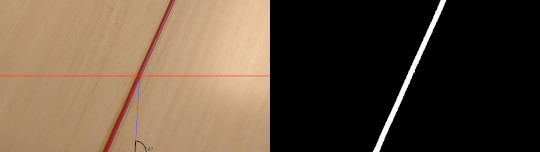
\includegraphics[width=1.0\columnwidth]{line_trace.jpg}
    \caption{Visualization of line following algorithm}
    \label{fig:mv_frame}
\end{figure}
\\ \\
% Step 3
To find the centroid of this binary image the \emph{moment} is calculated. The image moment is in some sense analogous to the concept of \emph{center of mass} used in physics. It is defined as
\begin{equation}
m_{p q}=\int_{-\infty}^{\infty} \int_{-\infty}^{\infty} x^{p} y^{q} I(x, y) \mathrm{d} x \mathrm{~d} y
\end{equation}
where $I(x,y)$ denotes the intensities of the image \cite{moment}.
This formula is discretized in order to be usable with an array of pixels
\begin{equation}
M_{p q}=\sum_{x} \sum_{y} x^{p} y^{q} I(x, y).
\end{equation}
The center of the image in the horizontal direction is then given by
\begin{equation}
    \bar{x} = \frac{m_{10}}{m_{00}}.
\end{equation}
\\ \\
% Step 4
All that remains to do is to calculate the angle between the horizontal axis and the line drawn between the point $(\bar{x}, y_0)$ and the base of the robot, denoted as $(x_r, y_r)$.
The angle $\alpha$ is given by
\begin{equation}
    \alpha = \tan^{-1}\left(\frac{y_0 - y_r}{\bar{x} - x_r}\right).
\end{equation}
The angle output is visualized in figure \ref{fig:mv_frame}.
This process is repeated for every captured frame and will produce a continuous stream of angles which can then be used by other components of the robot.

\section*{QR Code Reader}
In order to provide the robot with additional positional information QR codes are used.
The basic QR code functionality is provided with the use of the \emph{ZBar}\cite{zbar} library.






As with the line following algorithm each frame is processed and scanned for QR codes.
If a QR code is found in the input image the contents of the QR code, the position of the QR code and the cardinal direction from which the QR code is approached is sent as a message to be received by the other components of the robot.




\section*{Pathfinding}
To autonomously navigate between different points a pathfinding system is used. 
% Does this go under MV or some other base movement section?
Each QR code contains information of the form $\{x,y\}$, where $x$ and $y$ are the Cartesian coordinates of the QR code in the grid.
An internal representation of the entire grid is stored in the form of an adjacency matrix.
Dijkstra's algorithm is used to find the shortest path between two different coordinates in the grid. 

Calculating which direction the robot must turn to reach the next coordinate in the path is done using the relative position of the current and next QR code together with the direction from which the robot is approaching the current QR code.
First the angle between the two adjacent QR codes relative the horizontal axis of the grid is calculated.
Then the angle from which the robot is approaching the QR code is added to the angle between the QR codes.
This sum then represents the angle which the robot must turn to align itself to the next QR code in the path.

Once the robot is aligned a new line following procedure is started until the robot reaches the next QR code. This process is then repeated until the destination is reached.
